\documentclass{article}
\usepackage{amsmath}
\usepackage{xcolor}
\usepackage{amsthm}
\usepackage{graphicx}
\usepackage{hyperref}
\usepackage{datetime}
\usepackage{outlines}

\newdateformat{monthyeardate}{\monthname[\THEMONTH] \THEYEAR}

\newcommand{\newmarkedtheorem}[1]{%
  \newenvironment{#1}
    {\pushQED{\qed}\csname inner@#1\endcsname}
    {\popQED\csname endinner@#1\endcsname}%
  \newtheorem{inner@#1}%
}

\theoremstyle{definition}
%\newtheorem{eg}{Example}[section]
\newmarkedtheorem{eg}{Example}[section]
\newtheorem{observation}{Observation}[section]
\newtheorem{define}{Definition}[section]
\theoremstyle{plain}
\newtheorem{proposition}{Proposition}[section]
\newtheorem{theorem}{Theorem}[section]
\newtheorem{assump}{Assumption}[section]
\newtheorem{remark}{Remark}[section]

\title{Generalized Problem}
\author{Jeroen van Riel}
\date{\monthyeardate\today}

\begin{document}

\maketitle

\section{Platoon Forming Algorithms}

Let us start by briefly recalling the work by Marko and Rik on the analysis of
platoon forming algorithms \cite{timmermanPlatoonFormingAlgorithms2021}. They
consider a single intersection vehicle control problem in which arriving
vehicles are approaching the intersection from different lanes and need to be
guided safely accross the intersection in some efficient manner (minimizing some
global measure of delay and acceleration). They propose to solve this problem in
two stages. In the first stage (\textit{platoon forming algorithm}), a
\textit{polling policy} determines the order in which vehicles cross the
intersection. Given this decision, precise vehicle trajectories can be computed
efficiently as the second stage (\textit{speed control algorithm}).

The motivation for studying our single intersection scheduling problem has been
based on the above decomposition. Given a feasible schedule, we assume that
trajectories can be efficiently computed. Up till now, we have assumed that all
vehicle arrivals are known upfront, in which case the problem can be essentially
reduced to an \textit{offline} scheduling problem. When vehicle arrivals are
revealed to the traffic controller over time, we are dealing with some kind of
\textit{online} problem. In this case, note that it might be beneficial to
recompute (parts of) the trajectories upon new vehicle arrivals. An interesting
question is whether methods based on the two-stage decomposition are still
possible/sensible in the online case.

\begin{define}[Definition 3.1 from \cite{timmermanPlatoonFormingAlgorithms2021}]
  \label{def:regular}
  A polling policy is \textit{regular} if an arrival in a queue does not change
  the \textit{order} of service of all currently present vehicles, i.e. the new
  arrival is inserted somewhere in the order of service of all waiting vehicles.
\end{define}

The work of Marko and Rik provides a positive answer to this question under the
assumption that the polling policy is \textit{regular} (in terms of the
disjunctive graph, we could say that the currently fixed disjunctive arcs are
not changed upon arrival of new vehicles). However, in general, it is not clear
to me whether optimal policies can always be decomposed in similar ways. To
study this question further, we would first need a clearer understanding of the
general problem.

\section{General Traffic Control Problem}
\label{sec:general}

% vehicles moving through a graph and position encoding
Let us provide a rough sketch of a more general vehicle control problem on a
network of intersections, without assuming any structure on the solution
procedure like above. Consider a very abstract problem in which vehicles
represented as little dots are moving over a graph in a continuous fashion.
Vehicles arrive to the graph over time and need to follow a fixed route towards
a final node, where the vehicle leaves the system. The goal of the controller is
to determine how vehicles move exactly along their route, while satisfying some
constraints on the interaction between moving vehicles that stem from safety
considerations. In some sense, this is very reminiscent of models common in
train scheduling literature.

% routes and position in network
Recall our definition of the traffic network graph $G$ with internal and
external nodes. Again, let
\begin{align*}
  R_{j}(0), R_{j}(1), \dots, R_{j}(n_{j}), R_{j}(n_{j}+1)
\end{align*}
denote the route of vehicle $j$ and assume that vehicle $j$ arrives at external
node $R_{j}(0)$ at time $t_{j}^{0}$, assumed to be random. Let $x_{j}(t)$ denote
the position of vehicle $j$ on its route $R_{j}$ at time $t \geq t_{j}^{0}$. We
also use the notation $x_{ij}(t)$ to denote the position on the lane on the
route of $j$ leading to the $i$th intersection on its route, so we have
\begin{align}
  x_{ij}(t) = x_{j}(t) - \sum_{k=0}^{i-2} d(R_{j}(k), R_{j}(k+1)) .
\end{align}
Furthermore, let $v_{j}(t)$ and $a_{j}(t)$ denote the speed and acceleration,
respectively, of vehicle $j$ at time $t$.

\begin{figure}[b]
  \centering
  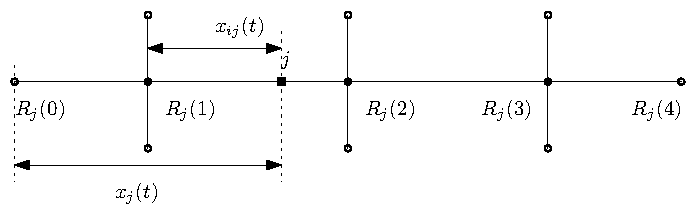
\includegraphics[width=0.9\textwidth]{figures/general_traffic_model.pdf}
  \caption{Illustration of a network of intersections with the position of some
    vehicle $j$ given in two ways.}
  \label{fig:general-model}
\end{figure}

% simple example
\begin{eg}
  Consider the network of intersections in Figure~\ref{fig:general-model}.
  Suppose vehicle $j$ is already in the network and assume $t$ is such that
  \begin{align}
    d(R_{j}(0), R_{j}(1)) < x_{j}(t) < d(R_{j}(0), R_{j}(1)) + d(R_{j}(1), R_{j}(2)) ,
  \end{align}
  then we say that vehicle $j$ is driving on the lane between the first and
  second intersection on its route (recall that only the $n_{j}=3$ nodes in the
  middle are considered to be intersections). Furthermore, the exact position on
  this lane is given by
  \begin{align}
    x_{2j}(t) = x_{j}(t) - d(R_{j}(0), R_{j}(1)) .
  \end{align}
\end{eg}


% trajectory constraints: smoothness, velocity and acceleration
The task of the traffic controller is to determine trajectories $x_{j}$ (or
equivalently either $v_{j}$ or $a_{j}$) satisfying some kind of smoothness and
safety constraints. For example, we may impose maximum/minimum speed constraints
\begin{align}
    v_\text{min} \leq v_j(t) \leq v_\text{max}
\end{align}
and acceleration constraints
\begin{align}
    a_\text{min} \leq a_j(t) \leq a_\text{max} .
\end{align}


% lane switching: merge point (head of common path)
Given a node $i$, we will use $t_{ij} = t_{ij}(x_{j})$ to denote the time when
vehicle $j$ crosses $i$, which of course depends on the chosen trajectory
$x_{j}$. Between crossing of vehicles from different lanes, we enforce a
\textit{safe lane-switching} time $s_{\text{lane}}$. Recall the definition of a
\textit{merge point}. At each merge point $i$ of each path $P \in P_{jl}$ for
all pairs of distinct vehicles $\{j,l\}$, we require that either
\begin{align}
  t_{ij} + s_{\text{lane}} \leq t_{il} \; \text{ or } \; t_{il} + s_{\text{lane}} \leq t_{ij} .
\end{align}

% following distance and overtaking: tail of common path
When two vehicles $j$ and $l$ are driving on the same lane we require some
minimum \textit{safe following distance} $d_{\text{follow}}$. Recall the
definition of \textit{common paths} $P_{jl}$. For all pairs of distinct vehicles
$\{j,l\}$, for each common path $P = (i_{1}, \dots, i_{L}) \in P_{jl}$, we
require for each intersection $i \in P$ that
\begin{align}
  \label{eq:following-distance-constraint}
  x_{ij}(t) + d_{\text{follow}} \leq x_{il}(t) \; \text{ or } \; x_{il}(t) + d_{\text{follow}} \leq x_{ij}(t)
\end{align}
for all $t$ in the time interval when both vehicles are driving on the common
path. When we do not allow vehicles to overtake each other, exactly one of the
inequalities must hold for the entire common path.

% unifying (to time domain)
For simplicity, the two types of constraints were stated in terms of time and
distance, respectively, which is not the most general approach. To illustrate,
we transform constraints~\eqref{eq:following-distance-constraint} to an
equivalent version in the time-domain. Defining the inverse of $x_{j}$ as
\begin{align}
  x_{j}^{-1}(x) = \inf \{ t: x_{j}(t) = x \} ,
\end{align}
we could instead have required
\begin{align}
  x_{j}^{-1}(x) + s_{\text{follow}} \leq x_{l}^{-1}(x) \; \text{ or } \; x_{l}^{-1}(x) + s_{\text{follow}} \leq x_{j}^{-1}(x) ,
\end{align}
for all positions $x$ on the common path. Furthermore, we might want to
have safe head-times that depend on the speeds of the involved vehicles.

\section{Optimization setting}

Let us now consider more precisely how the controller interacts with the system
defined above. First of all, we need to make some additional assumptions on the
random vehicle arrivals at external nodes. Like
\cite{limpensOnlinePlatoonForming2023} (Section 3), we assume vehicle arrivals
are \textit{safe}, which roughly means that safe following times need to be
respected between consecutive arrivals. More precisely, we require that
\begin{align}
  |t_{j}^{0} - t_{l}^{0}| \geq s_{\text{follow}} ,
\end{align}
for all pairs of vehicles $\{j,l\}$ arriving to the same external node.

\begin{figure}
  \centering
  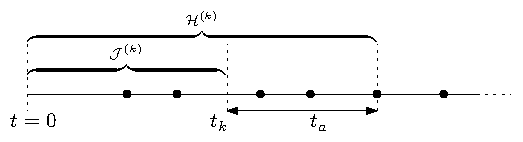
\includegraphics[width=1.0\textwidth]{figures/sequential-decision-process.pdf}
  \caption{Illustration of some decision epoch $t_{k}$ and the corresponding set
    of vehicles under control and the visible horizon. The dots represent vehicle
    arrival times $t_{j}^{0}$.}
  \label{fig:sequential-decision-process}
\end{figure}

In general, at some time $t$, we assume that the controller knows the arrival
times of vehicles
\begin{align}
  \mathcal{H}_{t} = \{ j : t_{j}^{0} \leq t + t_{\text{a}}\} ,
\end{align}
for some non-negative look-ahead time $t_{\text{a}}$. We call this set of
vehicles (with their corresponding arrival times) the \textit{visible horizon}
of the controller. Similarly, let the set of vehicles in the system at time $t$
be denoted by
\begin{align}
  \mathcal{J}_{t} = \{ j : t_{j}^{0} \leq t \} .
\end{align}
Ignoring for now that vehicles eventually leave the system, we say that
$\mathcal{J}_{t}$ are precisely the vehicles \textit{under control} of the
traffic controller.

Note that the only uncertainty in the system stems from the random arrival times
of vehicles. Once trajectories are determined, the dynamics of the system are
completely deterministic as long as $\mathcal{H}_{t}$ does not change.
Therefore, the only sensible decision epochs to consider are the points in time
$t_{k}$ whenever $\mathcal{H}_{t}$ changes, i.e., when new information becomes
available, see Figure~\ref{fig:sequential-decision-process} for an illustration.
Whenever this happens, the controller needs to compute a trajectory for the
newly arrived vehicles, and is free to revise the trajectories of the vehicles
that are already in the system. However, these updated trajectories need to
respect the trajectories that have been followed up till that point.

Let us make the sequential decision process sketched above a little bit more
precise. To simplify notation, we define
$\mathcal{J}^{(k)} = \mathcal{J}_{t_{k}}$ and
$\mathcal{H}^{(k)} = \mathcal{H}_{t_{k}}$. Let the \textit{state} of the system
at time $t_{k}$ be represented by the sets
\begin{align}
  s_{k} = (\{(t_{j}^{0}, R_{j})\}_{j \in \mathcal{H}^{(k)}}, \;
  \{(x_{j}^{(k-1)}(t_{k}), v_{j}^{(k-1)}(t_{k}), a_{j}^{(k-1)}(t_{k}))\}_{j \in \mathcal{J}^{(k)}} ) .
\end{align}
The controller needs to compute a set of trajectories
\begin{align}
a_{t} = \{ x_{j}^{(k)}\}_{j \in \mathcal{H}^{(k)}} ,
\end{align}
which are functions of $t \geq t_{j}^{0}$, satisfying the constraints from the
previous section and the additional constraints
\begin{subequations}
\begin{align}
  x_{j}^{(k)}(t_{k}) = x_{j}^{(k-1)}(t_{k}), \\
  v_{j}^{(k)}(t_{k}) = v_{j}^{(k-1)}(t_{k}), \\
  a_{j}^{(k)}(t_{k}) = a_{j}^{(k-1)}(t_{k}),
\end{align}
\end{subequations}
for the vehicles $j \in \mathcal{J}^{(k)}$ that were already under control,
guaranteeing in some sense the \textit{continuation} of the updated
trajectories.

From the above discussion, it should be clear that the transition to the next
state $s_{k+1}$ is particularly simple. The arrivals that happen at
$t_{k+1} + t_{a}$ are simply added to the visible horizon and the positions,
speeds and accelerations follow directly from the determined trajectories
$a_{t}$.

% TODO: vehicles leaving the network (could choose to let them stay at R_j(n_j))

% objective
We still have to define an objective to compare the performance of different
controllers. Measures of how well the controller performs on some particular
sequence of arriving vehicles may be based on properties of the computed
trajectories. For example, we could relate some measure of energy consumption to
acceleration, or we can measure delay based on the crossing times $t_{ij}$. In
general, the optimization objective is the expected value of this measure, where
the expectation is taken over the distribution of the vehicle arrival process.

% horizon
Finally, we may distinguish between a finite-horizon problem with a finite
number of vehicles, or an infinite-horizon case, in which particular attention
needs to be paid to the definition of the optimizaton objective, e.g., we might
need to use discounting to avoid infinite sums.


\section{Scheduling approach}

Given the above problem formulation, we are now in a better position to explain
the class of approaches that are based on explicit scheduling.

At some decision epoch $t_{k}$, the controller generates the set of trajectories
as follows.
First of all, one of the main assumptions is that vehicles cross intersections at maximum speed.
Assuming that acceleration can change instantly, it takes
\begin{align}
  t_{\text{acc}} = \frac{v_{\text{max}} - v_{j}(t_{j}^{0})}{a_{\text{max}}}
\end{align}
time to reach maximum speed. In this time period, simple calculation shows that the vehicle has traveled
\begin{align}
  x_{j}(t_{\text{acc}}) = t_{\text{acc}} v_{j}(t_{j}^{0}) + t_{\text{acc}}^{2} a_{\text{max}} / 2 .
\end{align}
To simplify notation, let
\begin{align}
  d_{kj} = \sum_{i=0}^{k-1} d(R_{j}(i), R_{j}(i+1))
\end{align}
denote the distance of the $k$th intersection on the path of vehicle $j$.
Assume that initial speeds are such that
$x_{j}(t_{\text{acc}}) < d(R_{j}(0), R_{j}(1))$, the \textit{earliest possible
  crossing time} of vehicle $j$ for its $k$th intersection is simply
\begin{align}
  r_{kj} = t_{\text{acc}} + \frac{d_{kj} - x_{j}(t_{\text{acc}})}{v_{\text{max}}} .
\end{align}
Assuming that vehicles arrive at maximum speed allows us to simplify this to
\begin{align}
  r_{kj} = \frac{d_{kj}}{v_{\text{max}}} .
\end{align}
The basis of the scheduling approach is to first determine the crossing times
$y_{kj} \geq r_{kj}$ for $j \in \mathcal{H}^{(k)}$ and then use this as a
starting point to compute feasible trajectories that satisfy
$x_{j}(y_{kj}) = d_{kj}$. In general, it is not clear that feasible trajectories
always exist. The paper of Marko and Rik shows that it is possible in case of
one intersection.



\bibliography{references}
\bibliographystyle{ieeetr}


\end{document}
